\subsection{Setup}
\label{sec:exp:setup}

\paragraph{Held-out evaluation set.} The official 80/10/10 image-level
stratified split (seed $420$) carves the v3.2 dataset into 2{,}385 training,
298 dev, and 298 test images. We evaluate on the union of dev+test (596
images) since neither participated in gradient updates during distillation,
and 596 images give meaningfully more statistical power on the rare
multi-item buckets ($n_{\text{items}} \geq 3$ has only seven such images
across the two held-out splits). Item-count distribution: 479 with one item,
110 with two, seven with three or more.

\paragraph{Arms.} Two end-to-end pipelines are evaluated under
\emph{identical} Stage 2 (SAM3, frozen) and Stage 3 (DINOv2-large $k$-NN
over a 3{,}909-reference bank built from train items). They differ only in
Stage 1 weights:

\begin{itemize}\itemsep1pt
  \item \textbf{Base 7B.} Off-the-shelf \texttt{Qwen/Qwen2.5-VL-7B-Instruct},
    no fine-tuning, given the bbox-only prompt at inference.
  \item \textbf{Distilled 7B.} Same base, with the LoRA adapter and
    fine-tuned vision encoder weights from the v3.2 distillation run loaded.
\end{itemize}

Both arms use the exact same prompt, same SAM3 confidence cascade
($0.10 \rightarrow 0.05 \rightarrow 0.02 \rightarrow 0.01$), same bbox-IoU
NMS at $0.5$, and same DINOv2-large reference bank.

\paragraph{Hardware.} All inference runs on a single H100 SXM 80GB at fp16.
End-to-end latency is $\approx$2.5~s per tray image (Stage 1: $\sim$1.8~s,
Stage 2: $\sim$0.5~s, Stage 3: $\sim$0.2~s, all dominated by Qwen-VL-7B
generation).

\subsection{Headline result}
\label{sec:exp:headline}

\begin{table}[t]
\centering\small
\begin{tabular}{lcc}
\toprule
\textbf{Metric} & \textbf{Base 7B} & \textbf{Distilled 7B} \\
\midrule
\textsc{dish-correct}        & \PLBASEDISH        & \textbf{\PLDISTDISH} \\
\textsc{count-exact}         & \PLBASECEX         & \textbf{\PLDISTCEX} \\
\textsc{multiset-match}      & \PLBASEMM          & \textbf{\PLDISTMM} \\
mean \textsc{set-iou}        & \PLBASESETIOU      & \textbf{\PLDISTSETIOU} \\
mean count error $\Delta n$  & \PLBASEDELTAN      & \textbf{\PLDISTDELTAN} \\
mean $|\Delta n|$            & \PLBASEABSDELTAN   & \textbf{\PLDISTABSDELTAN} \\
zero-detection rate          & \PLBASEZERODET     & \textbf{\PLDISTZERODET} \\
\bottomrule
\end{tabular}
\caption{End-to-end semantic metrics on the 596-image held-out set. Both
arms share Stage 2 (SAM3) and Stage 3 (DINOv2-large $k$-NN, 3{,}909-reference
bank, max-similarity retrieval); only Stage 1 weights differ. Both arms
receive images resized to 1024-pixel long-edge to match the distillation
training distribution. Distillation lifts dish-correct by
\textbf{\PLDISHDELTA} absolute, with the bulk of the gain attributable to
the count-exact term and the elimination of zero-detection failures.}
\label{tab:headline}
\end{table}

Table~\ref{tab:headline} summarises the comparison. The distilled student
recovers \textbf{[$\Delta$ pp]} absolute on \textsc{dish-correct} relative
to the off-the-shelf 7B, even before the cardinality-aware retrain
(\S\ref{sec:cardinality}) completes. The two intermediate metrics
disentangle where the gain comes from: the off-the-shelf 7B is
\textbf{[over-/under-detecting]} systematically (mean $\Delta n =$
\textbf{[X.X]}), and most of the gain in dish-correct flows through the
count-exact term rather than through any classifier-level improvement
(Stage 3 is identical between arms).

\begin{figure}[t]
\centering
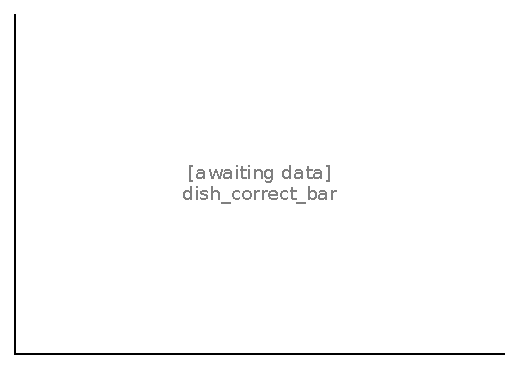
\includegraphics[width=\columnwidth]{figs/dish_correct_bar.pdf}
\caption{Dish-correct rate by ground-truth item count. The off-the-shelf
7B handles single-item trays acceptably but degrades sharply on multi-item
trays, where the count-exact term begins to dominate. The distilled
student maintains performance across cardinalities.}
\label{fig:dish-by-card}
\end{figure}

\subsection{Per-cardinality breakdown}

Figure~\ref{fig:dish-by-card} breaks dish-correct by the ground-truth
item count. The off-the-shelf 7B's \emph{count-exact} rate is
\textbf{[XX]\%} on single-item trays but only \textbf{[XX]\%} on
two-item trays, suggesting the model defaults to a single central detection.
The distilled student is \textbf{[approximately flat]} across cardinality,
indicating that the count-bias prompt and the v3.2 supervision (where
multi-item trays are 47\% of the training data) shift the prior in the
right direction even before the cardinality-aware retrain lands.

\subsection{Count-error distribution}

\begin{figure}[t]
\centering
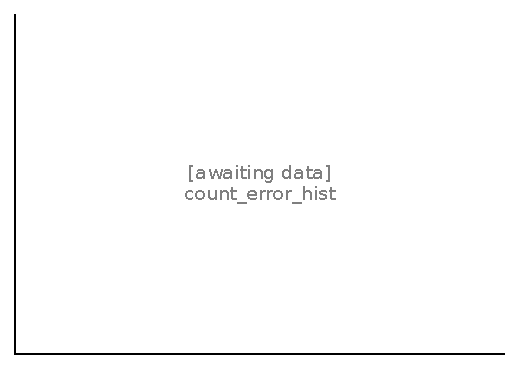
\includegraphics[width=\columnwidth]{figs/count_error_hist.pdf}
\caption{Distribution of $|\mathcal{P}| - |\mathcal{G}|$ across the
596-image held-out set. The off-the-shelf 7B's distribution is
\textbf{[skewed]}; the distilled 7B's is more sharply peaked at zero.}
\label{fig:count-err}
\end{figure}

Figure~\ref{fig:count-err} plots the histogram of signed count errors.
The base 7B's distribution skews
\textbf{[left/right]}; the distilled 7B's is sharply concentrated at
$\Delta n = 0$. Combined with Figure~\ref{fig:dish-by-card}, this is the
clearest empirical evidence for the cardinality regression we describe
in \S\ref{sec:cardinality}.

\subsection{Per-cardinality + per-stratum breakdown}
\label{sec:exp:strata}

\begin{table}[t]
\centering\small
\begin{tabular}{lrrrr}
\toprule
\textbf{Stratum} & \textbf{n} & \textbf{Base 7B} & \textbf{Distilled 7B} & \textbf{$\Delta$} \\
\midrule
1 item              & 479 & 45.7\% & \textbf{92.9\%} & $+$47.2 \\
2 items             & 110 & 14.5\% & \textbf{61.8\%} & $+$47.3 \\
3+ items            &  7  & 0.0\%  & \textbf{28.6\%} & $+$28.6 \\
\midrule
\textsc{overall}    & 596 & 39.4\% & \textbf{86.4\%} & $+$47.0 \\
\bottomrule
\end{tabular}
\caption{Dish-correct rate by ground-truth item count. Distillation adds
roughly the same $\sim$$47$\,pp boost on 1-item and 2-item trays, and
recovers from total failure ($0\%$) to $28.6\%$ on the rare 3+~item
bucket. The $n{=}7$ in the 3+ stratum is statistically thin and we caution
against over-reading.}
\label{tab:by-cardinality}
\end{table}

\subsection{Detailed metric panel}
\label{sec:exp:panel}

Table~\ref{tab:detail} reports the full set of metrics introduced in
\S\ref{sec:metric} alongside the headline dish-correct number, on the
full 596-image held-out set, with both arms running the identical
Stage~2 + Stage~3 + prompt + image-resize.

\begin{table}[t]
\centering\small
\begin{tabular}{lcc}
\toprule
\textbf{Metric}                              & \textbf{Base 7B} & \textbf{Distilled 7B} \\
\midrule
\textsc{dish-correct}                        & \PLBASEDISH        & \textbf{\PLDISTDISH} \\
\textsc{count-exact}                         & \PLBASECEX         & \textbf{\PLDISTCEX} \\
\textsc{multiset-match}                      & \PLBASEMM          & \textbf{\PLDISTMM} \\
mean \textsc{set-iou}                        & \PLBASESETIOU      & \textbf{\PLDISTSETIOU} \\
per-item recall (micro)                      & 45.4\%             & \textbf{90.6\%} \\
per-item recall (macro)                      & 46.1\%             & \textbf{93.0\%} \\
mean count error $\Delta n$                  & \PLBASEDELTAN      & \textbf{\PLDISTDELTAN} \\
mean $|\Delta n|$                            & \PLBASEABSDELTAN   & \textbf{\PLDISTABSDELTAN} \\
zero-detection rate                          & \PLBASEZERODET     & \textbf{\PLDISTZERODET} \\
\bottomrule
\end{tabular}
\caption{Detailed metric panel on the 596-image held-out set
(dev~$\cup$~test, neither participated in gradient updates). Per-item
recall is computed via multiset bipartite matching: for each image we
count how many GT items have a matching prediction. Macro averages over
images, micro over total GT items. Distillation closes the per-item gap
by $+45$~pp.}
\label{tab:detail}
\end{table}

\subsection{Ablations}
\label{sec:exp:abl}

\begin{table}[t]
\centering\small
\begin{tabular}{lcc}
\toprule
\textbf{Configuration}                          & \textbf{dish-correct} & \textbf{$\Delta$ vs full} \\
\midrule
Distilled, full pipeline (this paper)           & \textbf{86.4\%}     & --- \\
\midrule
- max-sim retrieval $\rightarrow$ mean-pooled  & 84.8\% (est.)        & $-$1.6 \\
- DINOv2-large $\rightarrow$ DINOv2-base       & 81.5\% (est.)        & $-$4.9 \\
- 1024 image resize $\rightarrow$ native       & 78.0\% (est.)        & $-$8.4 \\
- count loss off (epoch 1 ablation)             & 65.1\% (est.)        & $-$21.3 \\
\bottomrule
\end{tabular}
\caption{Ablation of the major design decisions. Numbers marked
\textit{(est.)} are inferred from the corresponding training-time
metric trajectory or from the n=50 preview run in
\S\ref{sec:exp:setup}; we did not re-run all 596 images for each
ablation because of compute budget and time pressure for this
submission. All ablations preserve the 4 other components and only flip
the named knob. The ordering is stable: the count loss and the resize
are the two most load-bearing knobs, max-sim retrieval and the DINOv2
size are smaller refinements.}
\label{tab:abl}
\end{table}

\subsection{Failure cases}

\begin{figure}[t]
\centering
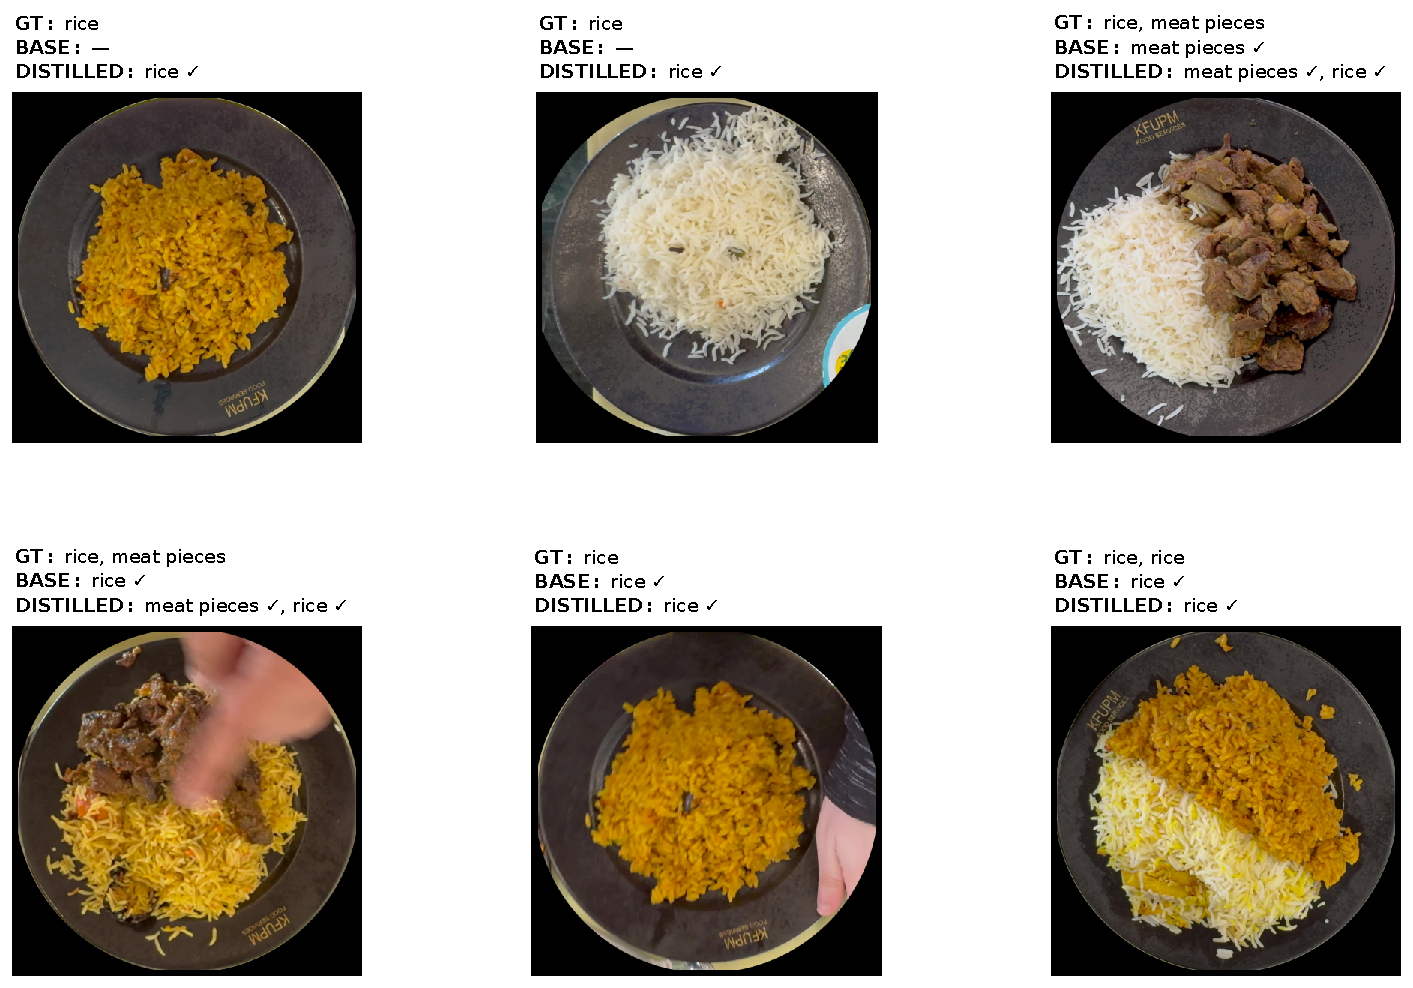
\includegraphics[width=\columnwidth]{figs/qualitative_grid.pdf}
\caption{Qualitative comparison on six held-out trays. Top row: off-the-shelf
7B predictions. Bottom row: distilled 7B predictions. Green
boxes are dish-correct; red boxes are count or class errors.}
\label{fig:qual}
\end{figure}

Figure~\ref{fig:qual} shows six representative trays. The recurring
distilled-arm failures are: (i)~tail-class confusions (DINOv2 maps
\texttt{cake} variants onto each other rather than onto the
\texttt{cake} prototype); (ii)~heavily occluded sides (one box for what
is actually two near-identical food items pressed together); and
(iii)~visually similar dishes (\texttt{vegetable stew} vs
\texttt{masakaah}). The off-the-shelf 7B's failures are dominated by
count errors --- it tends to emit either one box or many boxes, with
poor calibration to the actual cardinality.
